\providecommand{\main}{..}
\documentclass[\main/master.tex]{subfiles}
\begin{document}
\chapter{Methods and results}\label{chapter:Methods and results}

\section{System build}
\begin{figure}[htbp]
	\centering
	\fbox{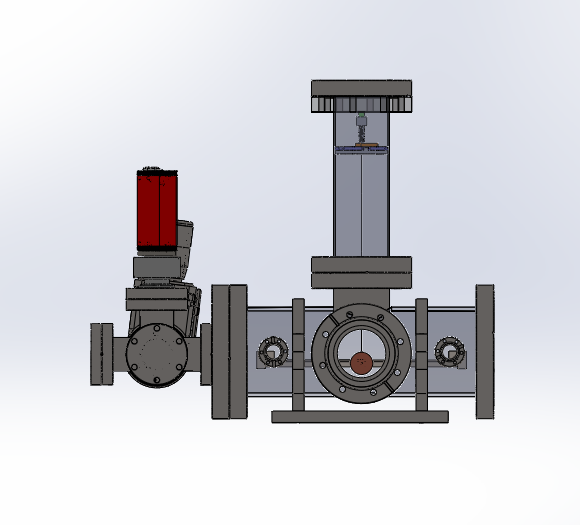
\includegraphics[scale=0.3]{\main/images/4 - methods and results/total_chamber.png}}
	\caption[Total chamber]{Total chamber}
	\label{fig:Total chamber}
\end{figure}
\FloatBarrier
\par\noindent
The experiment system was designed to minimize magnetic noises by avoiding capacitance and choosing low magnetic permeability materials.
\par\noindent
The torsional pendulum is placed inside a vacuum chamber, reducing Brownian motion, acoustic waves and friction. The vacuum chamber also reduces magnetic noise as a Faraday cage.
\par\noindent
The vacuum chamber is placed inside seismic box, farther reducing acoustic waves and magnetic noises from the environment.

\par\noindent
The experiment system was designed to minimize the outgassing rate, both by choosing low outgassing materials and avoiding air pockets in the devices. 
\par\noindent
Design of torsional pendulum and vacuum chamber was carried out using Solid Works.

\subsection{Torsional pendulum design}
\begin{figure}[htbp]
	\centering
	\fbox{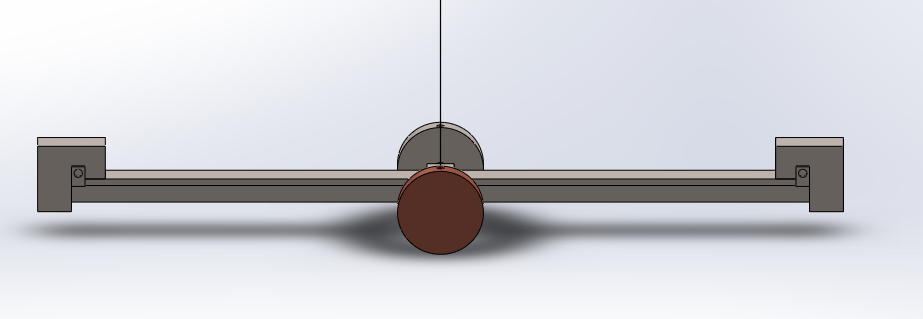
\includegraphics[scale=0.3]{\main/images/4 - methods and results/pendulum_front.png}}
	\caption[Torsion pendulum, front view]{Torsion pendulum, front view}
	\label{fig:pendulum front}
\end{figure}
\FloatBarrier
\subsubsection{Design constraints}
\par\noindent
The chosen pendulum dimensions are designed to balance two problems, to achieve high angle sensitivity to field (large string torsion coefficient $\kappa$) while having high mass sensitivity to angle (longer oscillation time period $T$). 
\par\noindent
As shown previously, for a torsional pendulum with length of $2l$, two identical masses $m$ on the sides, and a string with diameter $d$ and length $h$, where $I$ is the pendulum moment of inertia:
\begin{equation}
\kappa = \frac{G}{h} \frac{\pi d^4}{32}    \label{eqn:torsion_coefficient}
\end{equation}
\begin{equation}
T = 2\pi\sqrt{\frac{I}{\kappa}}= 2\pi\sqrt{\frac{2ml^2}{\kappa}}   \label{eqn:undamped_motion_equation}
\end{equation}
Longer string with smaller diameter results with a desired small string torsion coefficient $\kappa$. 
\par\noindent
In order to achieve a string with as small diameter as possible, tungsten string with high tensile strength was chosen. The high tensile strength allows a small diameter while overcoming suction forces when vacuum engine is working and holding the pendulum without tear. Tungsten is also vacuum compatible. The shear modulus $G$ for tungsten; 130-160 [Gpa]\cite{tungsten}.
\par\noindent
In order to minimize the magnetic noise in the measurements, the torsion pendulum was made out of stainless steel 316 (instead of stainless steel 304). Stainless steel 316 has a lower relative magnetic permeability $\mu_r$ \cite{SS316}.
\par\noindent
The experiment, is constructed using a front mirror, the angle displacement causes a mirror tilt. In order to minimize the magnetic noise, chosen mirror is made fully of metal (instead of coated glass). Having an Oxygen-free copper (OFC) mirror, while not officially vacuum compatible hopefully minimizes the vacuum outgassing.

\subsubsection{Design}
\par\noindent
The torsion pendulum angle tilt is measured using a mirror connected in front of the pendulum. The mirror is a part of an optical interferometer with which the mirror tilt could be determined.
\par\noindent
In order to balance the pendulum so the mirror would not have an initial downward tilt, beside the tilt caused by the gravity field. The pendulum center of mass needs to be adjusted. 
\par\noindent
The center of mass is adjusted using a matching mass of the mirror from behind, which balances the mirror weight.
\par\noindent
The matching mass $m_1$ has a similar weight and shape as the mirror $m_2$, both are connected to the pendulum via spring $w$ from their center. The spring enables accurate distance adjusting to prevent downward tilt.
\begin{figure}[htbp]
	\centering
	\fbox{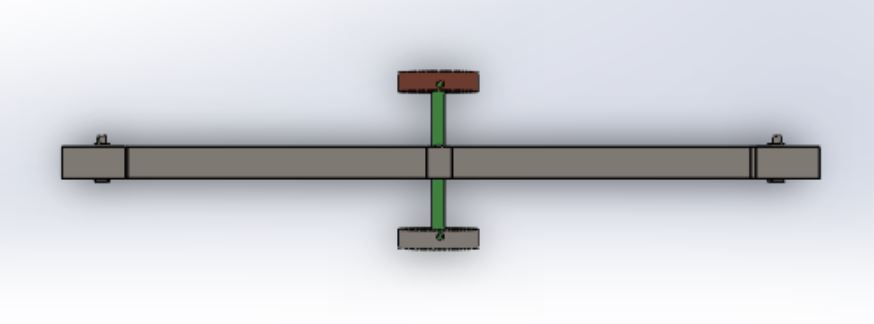
\includegraphics[scale=1.2]{\main/images/4 - methods and results/pendulum_top.JPG}}
	\caption[Torsion pendulum, top view]{Torsion pendulum, top view}
	\label{fig:pendulum top}
\end{figure}
\FloatBarrier 
\begin{equation}
\tau_y = 0 = m_1r_1g-m_2r_2g = m_1r_1g-m_2(w-r_1)g    \label{eqn:downward torque}
\end{equation}
\begin{equation}
\frac{m_1}{m_2} = \frac{w-r_1}{r_1}\approx 1   \label{eqn:downward torque}
\end{equation}
\subsubsection{Technical information}
\begin{easylist}
& Tungsten string;
&& made of 99.95\% pure Tungsten
&& length $h$ of 249 mm
&& diameter $d$ of 0.08 mm
& Torsional beam;
&& made of Stainless steel 316
&& length $2l$ of 218 mm
% && width of 10 mm 
%& & weight of 90 gram 
&& identical side masses weight $m$ 20.5 gram
& Mirror;
&& made of Oxygen-free copper (OFC), gold coated
&& diameter of 1 inch
\end{easylist}
\begin{easylist}
& results;
&& expected;
&&& $I = 0.487\cdot10^{-3}[kg\cdot m^2]$
&&& $\kappa = 2.1\cdot10^{-6}[\frac{N\cdot m}{rad}] - 2.6\cdot10^{-6} [\frac{N\cdot m}{rad}]$
&&& $T = 96[s] - 86 [s]$
&& experimental;
&&& $\kappa = 2.7\cdot10^{-6}[\frac{N\cdot m}{rad}]$
&&& $T = 84[s]$
\end{easylist}

\subsection{Vacuum chamber design}
\begin{figure}[htbp]
	\centering
	\fbox{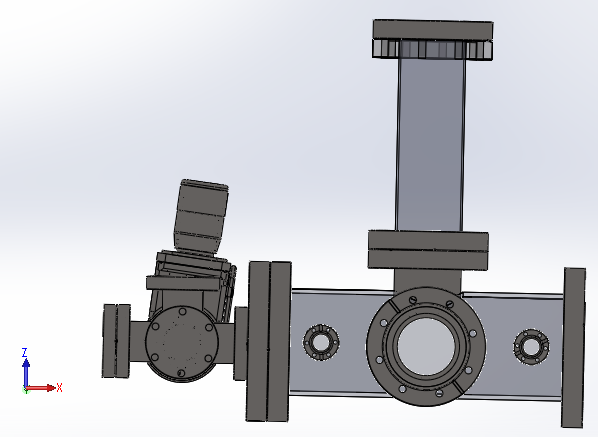
\includegraphics[scale=0.5]{\main/images/4 - methods and results/chamber_front.png}}
	\caption[Vacuum chamber, front view]{Vacuum chamber, front view}
	\label{fig:chamber front}
\end{figure}
\FloatBarrier

\par\noindent
Vacuum chamber build is two cylindrical tubes placed on each other with three view ports in front. The chamber has a 5-way which is connected to the vacuum engine and gauge.
\par\noindent
Vacuum chamber is bounded to the breadboard by an adjustable mount.
\par\noindent
Vacuum engine is connected to chamber through a valve, measurement is made when valve closed and engine off, to prevent rotation noise.

\subsubsection{Chamber viewports}
\par\noindent
Central viewport is in front of the pendulum's mirror, to measure the tilt angle. Two small viewports on the sides of the chamber are used by the noise damping system (PID) to damp noises. 
\par\noindent
The view ports are for 550-1100 nm, with about 98$\%$ power transmittance in the range.
\par\noindent
Central viewport has 68.3mm View diameter, and the distance from the mirror is 82 mm which is giving a full FOV of about $39^0$ degrees (instead of $90^0$ at interferometry).

\subsubsection{Pendulum mount}
\begin{figure}[htbp]
	\centering
	\fbox{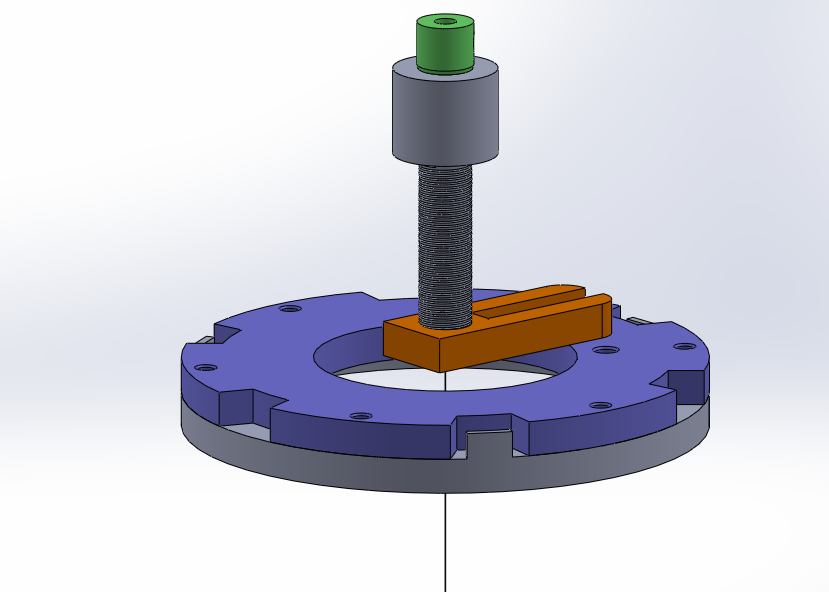
\includegraphics[scale=0.2]{\main/images/4 - methods and results/mount.png}}
	\caption[Pendulum mount]{Pendulum mount}
	\label{fig:mount}
\end{figure}
\FloatBarrier
\par\noindent
The upper tube of chamber is soldered with a base to which a mount is connected. The pendulum string is held via the mount.
\par\noindent
The mount is adjustable, enabling to adjust the pendulum's string length, so pendulum would be in front of viewports accurately. 

\subsection{Vacuum quality}
\subsubsection{pressure increase}
\par\noindent
Vacuum chambers are metallic chambers connected to a vacuum pump with pressure lower than the atmospheric pressure. The main limitations to vacuum quality maintenance are leakage $Q_L$ from the outside through the chamber and outgassing $Q_{des}$ inside the chamber (desorption of gas molecules from the material).
\par\noindent
Leaks and outgassing both increases the pressure at a constant rate over time, and are overcome by having a constant pump rate $Q_P$ (vacuum pump working constantly).   
\begin{equation}
Q_P = Q_L + Q_{des}  \label{eqn:vacuum_equilibrium}
\end{equation}
In this experiment due to the relatively large size and unique shape of the measurement equipment, the vacuum chamber is having both a large leak and outgassing rates. The sensitivity of the measurement does not allow having the pump working, causing pressure increase over time.
\subsubsection{minimized pressure increase}
\par\noindent
Vacuum chamber and measurement system were baked out to reduce outgassing, using resistive wire. 
\par\noindent
Bake out was carried for a weak at about $110 C^0$ achieving stable vacuum of about $2\cdot 10^{−4} [Torr]$ after cool down.
\par\noindent
The vacuum chamber was built using CF style vacuum Components, designed for ultra high vacuum, minimizing the leak rate.


\subsection{Noise reduction}
\subsubsection{Faraday cage}
\par\noindent
Faraday cage is a cage made by a continuous covering of a conductive material used to block external electromagnetic fields. The external electrical fields causes an electric charge distribution in the conductive cage without passing inside. Electric current decays exponentially with depth through the material.

\par\noindent
The cage blocks better the penetration of high frequency magnetic fields, depending on the material skin depth $\delta$ which determines the shield penetration depth for a defined frequency. Skin depth is dependent on the material electric resistivity $\rho$ and magnetic permeability $\mu$. 
\begin{equation}
\delta = \sqrt{\frac{2\rho}{(2\pi f)(\mu)} }    \label{eqn:skin depth}
\end{equation}

\subsubsection{Seismic box}
The measurement system is placed inside a seismic box which is a faraday cage with 76 mm thickness, blocking magnetic fields with $f \ge 30 [Hz]$ from the environment.
\par\noindent
The seismic box is both reducing acoustic waves and magnetic noises from the environment.
\subsubsection{Vacuum chamber}
The Vacuum chamber is a second faraday cage blocking magnetic noise from the electronic system placed inside the seismic box.
\par\noindent
Vacuum chambers are made of stainless steel 316 with approximately 3 mm thickness, making a faraday cage which blocks magnetic fields with $f\ge 20 [KHz]$ while reducing magnetic noises from lower frequency fields.
\par\noindent
As seen previously, Brownian motion, acoustic waves and friction are pressure dependent and are farther reduced by having vacuum.

\subsection{Noise reduction}
\par\noindent
After the desired vacuum is achieved, engine disconnected using the valve and engine turned off. The seismic box is closed, and waiting for the oscillations to damp down.


\par\noindent
ThePID is damping the noises, and after they are damped the measurement begins.






















\section{Proportional–Integral–Derivative (PID)}
\subsection{Damped oscillator}
PID controller can continuously calculates error value of an oscillator, to damp it to zero. If the defined set point is set to zero, the error is the measured process variable. The PID acts as friction, gradually working when the oscillations are at the maximum speed to slow them down, and remove the torque energy.
\begin{equation}
e(t) = \theta(t) = \theta   \label{eqn:error}
\end{equation}
\begin{equation}
\tau_{PID} = -\gamma\cdot\dot{\theta}   \label{eqn:friction_torque}
\end{equation}
The system is a damped oscillator, with an external force correction, which inserts torque to the oscillator.
\begin{equation}
\kappa\cdot\theta - \gamma\cdot\dot{\theta}  + I\cdot\ddot{\theta} = 0   \label{eqn:damped__pid_motion_equation}
\end{equation}
\begin{equation}
\gamma\dot{\theta}  = LF   \label{eqn:damped__pid_motion_equation}
\end{equation}
\begin{equation}
\dot{\theta} = \omega_0\theta_{max}sin(\omega_0 t +\phi)    \label{eqn:undamped_motion_equation}
\end{equation}
\begin{equation}
\dot{\theta}_{max} = \omega_0\theta_{max} = \theta_{max}\cdot\frac{2\pi}{T}    \label{eqn:undamped_motion_equation}
\end{equation}
\begin{equation}
\gamma  = \frac{LF_{max}}{\dot{\theta}_{max}} =\frac{LF_{max}T}{\theta_{max}2\pi}    \label{eqn:damped_pid_motion_equation}
\end{equation}
\begin{equation}
\tau =  \frac{2I}{\gamma}  \label{eqn:damping_time}
\end{equation}
The PID damping $\gamma$ and damping time $\tau$ depends on the initial oscillations angle. If the angle is too large compare to the inserted force, the system is extremely underdamped and the PID affect is negligible. The damping time would be infinite and the system would keep on oscillating.

\subsection{Control stability}
Using PID control does not guarantee optimal control or stability. The control system is aiming to achieve critical damping of the process. Well tuned control would a reach the desired set point fast and accurate, and also apply over time the necessary corrections to resist external forces trying to move variable from the set point.
\par\noindent
The controller response is its response to error. How much does the system overshoots a setpoint and the system oscillations. When controller gains are too high, instead of critical damping there is overdamping causing overshoot, due to the high gain the overshoot response overshoots to the other side, causing the system to be driven.
\subsection{Radiation pressure force}
The pendulum is cooled down using radiation pressure force. Fast modulated light source with high intensity cause a small controlled force. The difference between two light sources from both ends of pendulum adds a controlled small damping torque. 
\begin{equation}
F = \frac{2\eta\Theta}{{c}} \label{eqn:radiation force}
\end{equation}
\begin{equation}
\tau\approx d\Delta F = \frac{2d}{{c}} (\eta_1\Theta_1 -\eta_2\Theta_2) \label{eqn:radiation torque}
\end{equation}
The radiation pressure torque assuming light fields direction perpendicular to surface, $\Theta$ is the light source radiant flux [watt], and $\eta$ is the coupling efficiency. The center of mass distance from rotation axis $d$ of both forces is even.
\par\noindent
The setup could produce very small torques; light sources of 1 watt maximum power and 8bit modulation steps could produce nano-$N\cdot m$ to pico-$N\cdot m$ torques. 










\section{Modulated CW laser}

\subsection{Laser}


The laser is a high power coherent light source based on stimulated emission with narrow spectrum. Inside a cavity Electron is excited to a higher energy level, and forced by photon with the correct wavelength to be absorbed emitting coherent photon. The coherence allows focusing beam to a tight spot, and being collimated over long distances. Continuous wave (CW) laser are lasing constant output power over time.



\par\noindent
Usually the power output is stable but has oscillations due to having several longitudinal modes causing nano second scale oscillations, output power is steady when averaged over longer periods. Also, over long periods of time lasers have slight power oscillations due to temperature changes in the environment.
%The laser diode cavity face is rectangular, because of fabrication constraints. The rectangular face is causing cylindrical aberration, which   

\subsection{Acousto optic modulator}
Acousto Optic Modulator (AOM), uses the acousto-optic effect to diffract and shift the frequency of light using RF waves. An oscillating electric signal drives a piezoelectric transducer to vibrate causing RF waves, the transducer attached to a material. This causes sound waves in the material, and periodic index modulation causing a Bragg grating. Incoming light scatters off the grating and due to Bragg diffraction comes at Bragg angle.
\begin{equation}
\theta_b = sin(\theta_b)\approx \frac{\lambda}{2n\Lambda} \label{eqn:energy-mass-equivalence-relation}
\end{equation} 
$\Lambda$ is the RF wavelength, $\lambda$ is the light source wavelength. 
\par\noindent
Since all parameters constant, modulation angle is constant, and possible modulation speed is nano seconds. Giving a stable fast modulation method for CW laser.


\section{Modulated LED}
\subsection{Arduino}
Arduino is an open-source microcontroller board used for building low cost and simple digital devices and circuits. Each microcontroller contains a microprocessor, controller, serial communication interface and is equipped with digital and analog input/output pins. The microcontrollers could be operated as stand alone or connected to computer through serial communication. 
\par\noindent
The Arduino Mega 2560, based on the ATmega2560 8-bit controller, is equipped with 16 MHz crystal oscillator (clock) and 15 PWM outputs pins. Arduino doesn't have analog output, but is simulates analog output using Pulse Width Modulation.
\par\noindent
The controller switches the output signal between the board Vcc (which is a digital 5[V]) and off, generating a square wave.
Repeating the pattern fast enough results in an analog signal as if the signal is a steady voltage. The time signal duration called the pulse width. Controller is modulating with clock the pulse width, changing the ratio time signal is on compare to off. 
\par\noindent
Output voltage is determined by that ratio, which is called duty cycle. 100\% duty cycle meaning power is always on and output is the full Vcc, 0\% power off and 50\% signal is on and off equally resulting with output of half. 
\par\noindent
The method enables generating signals between board Vcc and off. Signal resolution limited by the microcontroller resolution (8-bit). Due to the fast Arduino clock possible signal modulation frequency is up to 500Hz.
\par\noindent
Since clock is connected to all PWM pins, they are in sync. When all pins have the same duty cycle, they all have the same voltage over time. At every point in time they could be looked at as a constant voltage supplies compare to each other, allowing to connect them in series and increase the output current up to 1[A]. 
\subsection{Light Emitting Diode (LED)}
The light emitting diode (led) is a high power long lifetime light source semiconductor based. The led is emitting light when current flows through. Led could be modulated at up to 100MHz. The initial opening angle of a led source varies between 45 to 120 degrees. The emitted light is incoherent in width meaning it's hard to focus it to a point (not diffraction limited). The emitted light is incoherent in length causing wide band spectrum.

\par\noindent
Forward voltage is applied causing electron injection and recombination with holes. The recombination is releasing energy in form of spontaneous emission photons. The modulation limitation is due to the electrons life time before recombination. The led power is proportional to the current flows through, Shockley diode equation for p-n junction defines the current relation to the diode voltage. In high enough values the power could be approximated by linear approximation of the diode voltage.
\begin{equation}
P\propto e^{\frac{q}{kT}\cdot V_d}\label{eqn:energy-mass-equivalence-relation}
\end{equation}
In order to overcome the led uncoherent profile and large opening angle, light was transferred through a light guide. Light guides are pipes made of thin filaments causing internal reflections used for directed transmission of luminous energy. Light guides are used to illuminate small areas, regardless of the spectral characteristics of the light source. They mainly depend on the cross sections of entrance and exit and the length. Making them ideal to overcoming focusing problems.
\par\noindent
Connecting a high power led to Arduino, enables fast real-time controlled modulation of high power led with about 2ms speed. The light arrives to pendulum through a light guide allowing to assume beam variation through the surface negligible.The light is controlled through a PID and applies a torque.
\par\noindent
Since the led power could be approximated using linear approximation, the power modulation is proportional to the Arduino duty cycle. That allows to control the linear approximation of the power output by changing the PID gain values.  
\par\noindent
we assume we can neglect the oscillations between two sides...



\begin{figure}[htbp]
	\centering
	\fbox{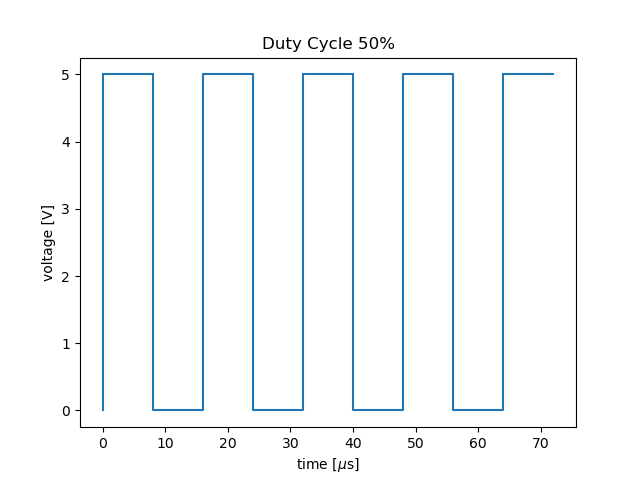
\includegraphics[scale=0.5]{\main/images/devices/duty50.png}}
	\caption[Duty cycle 50\%]{Duty cycle 50\%  - signal is on and off equal times}
	\label{fig:duty50}
\end{figure}
 
\begin{figure}[htbp]
	\centering
	\fbox{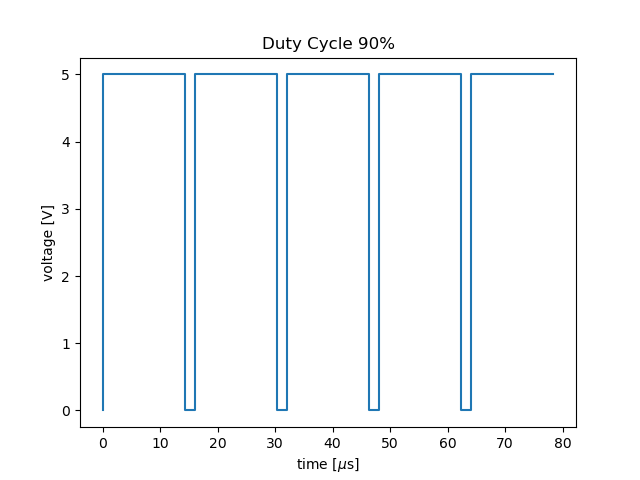
\includegraphics[scale=0.5]{\main/images/devices/duty90.png}}
	\caption[Duty cycle 90\%]{Duty cycle 90\% - 90\% of the time signal on, equivalent to 90\% of the full Vcc signal}
	\label{fig:duty90}
\end{figure}














\section{pid operate (algorithm)}
\section{laser +aom +amp}
\doublespacing



\section{Overshoot}
Overshoot is when output signal or function exceeds the target value. The response signal is not accurate compare to target. In control theory there are two wanted conflicting properties; an accurate response (small overshoot), and small risetime (fast response). 
\par\noindent
Overshoot is usually measured in percentage overshoot (PO). For second order systems, such as damped oscillators PO is a function of the damping ratio $\xi$. 


\begin{equation}
PO = 100\cdot e ^{\frac{-\xi\pi}{\sqrt{1-\xi^2}}} = \frac{output-target}{target}   \label{eqn:percentage_overshoot}
\end{equation}
 
\section{Accuracy}
\end{document}